\documentclass{article}
\usepackage[tc]{titlepic}
\usepackage{xcolor}
\usepackage{float}
\usepackage{graphicx}
\usepackage{tipa}
\usepackage{pagecolor,lipsum}
\usepackage{amsmath}
\usepackage{amsfonts}
\usepackage{fullpage}
\usepackage{amssymb}
\usepackage{amsthm}
\usepackage{centernot}
\usepackage{listings}
\usepackage{tikz, ifthen}
\usepackage{enumitem}
\usepackage{forest}
\usetikzlibrary{positioning}

\usetikzlibrary{calc}

\newtheorem{theorem}{Theorem}
\newtheorem{defintion}{Definition}
\newtheorem{collorary}{Collorary}
\newtheorem{example}{Example}
\newtheorem{remark}{Remark}
\newtheorem{note}{Note} 
\newcommand{\arr}{\rightarrow}
\tikzset{main node/.style={circle,fill=blue!20,draw,minimum size=1cm,inner sep=0pt},} 

\begin{document}
\section{Algorithms are important for interview}

\section{SQL}
\subsection{Innter join, outer join}
\begin{itemize}
 \item Innter join, outer join 
 \item foreign key
 \item Database Sharing, indexing
 \item noSQL, key and value 
\end{itemize}

\section{Coin Change Problem}
\subsection{This is fun question}
\begin{example}
Given a set of coins and an integer $S$, find all the combination of coins are added up to the integer $S$.\\
$[2, 4, 3]$ and $S$

\subsection{Find the minimum number of coins are added up to the $S$}

\end{example}

\section{Quick Sort}
QuickSort is important in sorting algorithms family because the runtime of QuickSort is
$\mathcal{O}(n\log{}n)$ on average case and the memory cost is $\mathcal{O}(1)$, it means you don't need a buffer to hold the elements.
Although the worst runtime is $\mathcal{O}(n^2)$, it is very unlikely case in real life data.
\subsection{Quick Sort Recursion}
\begin{itemize}
 \item[] choose the pivot and partition array to two parts 
 \item[] all the elem are less than pivot are on left part excluding the pivot
 \item[] all the elem are greater than pivot are on right part excluding the pivot
\end{itemize}
\pagebreak
\subsubsection{Quick Sort Partition}
The tricky part of quick sort is how to partition an array to two parts.
A Naive way is go through the element one by one and copy all the elements are less than the pivot to an array and do the same for the elements are greater than the pivot. 
The above solution works but the memory cost is $\mathcal{O}(n)$

There is in-place solution for partition. \\

\begin{minipage}{\linewidth}% to keep image and caption on one page
\makebox[\linewidth]{%        to center the image
  \includegraphics[keepaspectratio=true,scale=0.2]{/Users/cat/myfile/github/image/quicksort3.png}}
\end{minipage}

\begin{itemize}
\item Let $p$ to be the index of \textbf{array} that tracks the element is greater than the pivot. 
\item Let $i$ to be the index from $0$ to $len(\textbf{array})-1$ 
\item $p$ and $i$ are both start from $0$ and advance at the same time. 
\item If $p$ is greater than the pivot, $p$ stop increasing. Otherwise swap $p$ and $i$ 
\end{itemize}

\begin{lstlisting}[
  mathescape,
  columns=fullflexible,
  basicstyle=\fontfamily{lmvtt}\selectfont,
]
    partition array 
        p = 0
        for(int i=0; i<array.length; i++)
            if(array[i] <= pivot)
                swap(p, i)    
                if(p < array.length - 1)
                    p++

    return p
\end{lstlisting}

\pagebreak
\subsubsection{Preorder pattern in Quick Sort}
The recursion part of the quick sort is using preorder traveral.
\begin{verbatim}
    preorder node r
        if r is not null
            r.data
            preorder r.left
            preorder r.right

    quicksort array lo hi
        if lo < hi
            p = partition array lo hi
            quicksort array lo p-1
            quicksort array P+1 lo

\end{verbatim} 

\subsection{When is the runtime $\mathcal{O}(n^2)$}
\begin{example}
Given a sorted list $[1, 2, \dots n]$ and the right most element are chosen as pivot \\
then $[1, 2,\dots n-1][p=n]$ is generated in the first partition. So we have following \\
$[1, 2, \dots n-1][p=n]$ \\
$[1, 2, \dots n-2][p=n-1][p=n]$ \\
$[1, 2, \dots n-3][p=n-2][p=n-1][p=n]$ \\ \\
Every step, only the left part of the array which is the full array excluding the pivot are shuffled. \\
Thereforce, the runtime is $\mathcal{O}(n^2)$

%\begin{figure}
%\centering
%\includegraphics[scale=0.4]{/Users/cat/myfile/github/graphviz/quicksort.pdf}
%\caption{Quick Sort Recursion}
%\end{figure}
\end{example}

\subsection{Quick Sort Iteration}
Use preorder iteration algorithm $\arr$ one stack

\subsubsection{Implementation} 

% gf http://tex.stackexchange.com/questions/150965/insert-symbols-inside-verbatim-mode-latex
% \usepackage{listings}
% listings is similar to verbatim, but it detects math mode
% -------------------------------------------------------------------------------- 
\begin{lstlisting}[
  mathescape,
  columns=fullflexible,
  basicstyle=\fontfamily{lmvtt}\selectfont,
]
preorderIteration Node r
    while(r is not null or stack is not empty) 
        if r is not null
            print r.data
            stack.push r    $\quad$ // f(r $\leftarrow$ r.left)
            r = r.left
        else
            n = stack.pop()
            r = n.right     $\quad$ // f(r $\leftarrow$ r.right)
\end{lstlisting}

\pagebreak
\section{Binary Tree} 
\subsection{preorder}
\subsubsection{Application}
more info
\begin{lstlisting}[
    mathescape,
    columns=fullflexible,
    basicstyle=\fontfamily{lmvtt}\selectfont,
    ]
        preorder node r
            stack
            while r not null or stack is not empty
                if r not null
                    print r.data
                    stack.push r
                    r = r.left
                else
                    n = stack.pop
                    r = r.right

\end{lstlisting} 

\subsection{Inorder}
\begin{lstlisting}[
    mathescape,
    columns=fullflexible,
    basicstyle=\fontfamily{lmvtt}\selectfont,
    ]
        inorder node r
            stack
            while r not null or stack is not empty
                if r not null 
                    stack.push r
                    r = r.left
                else
                    n = stack.pop
                    print n.data
                    r = r.right

\end{lstlisting} 

\subsection{postorder}
\begin{lstlisting}[
    mathescape,
    columns=fullflexible,
    basicstyle=\fontfamily{lmvtt}\selectfont,
    ]
        postorder node r
            stack s1 s2
                if r not null
                    s1.push r
                    while s1 is not empty
                        n = s1.pop
                        if n.left is not null
                            s1.push n.left
                        if n.right is not null
                            s1.push n.right
                        s2.push n

                    while s2 is not empty
                        print s2.pop

\end{lstlisting} 

%\begin{minipage}{\linewidth}% to keep image and caption on one page
%\makebox[\linewidth]{%        to center the image
%\includegraphics[keepaspectratio=true,scale=0.2]{/Users/cat/myfile/github/image/postorder4.png}}
%\end{minipage}
% gf http://tex.stackexchange.com/questions/8625/force-figure-placement-in-text 

\pagebreak
\section{path problem}
\textbf{Find the all paths from two given nodes} \\
\begin{center}
  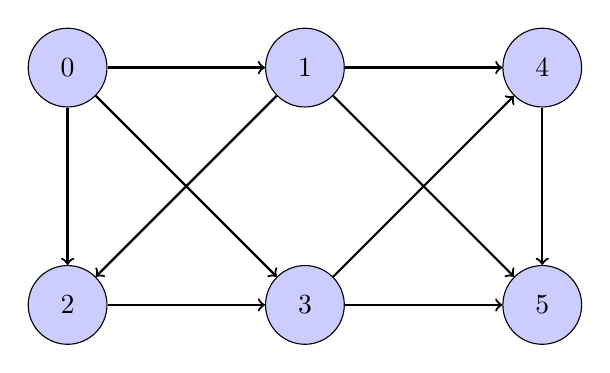
\begin{tikzpicture}
    \begin{scope}[xshift=4cm]
    \node[main node] (0) {$0$};
    \node[main node] (1) [right = 2cm  of 0] {$1$};
    \node[main node] (2) [below = 2cm  of 0] {$2$};
    \node[main node] (3) [right = 2cm  of 2] {$3$};
    \node[main node] (4) [right = 2cm  of 1] {$4$};
    \node[main node] (5) [below = 2cm  of 4] {$5$};

    \path[draw,thick]
    (0) edge[->] node {} (1)
    (1) edge[->] node {} (4)
    (4) edge[->] node {} (5)
    (1) edge[->] node {} (5)
    (0) edge[->] node {} (3)
    (3) edge[->] node {} (4)
    (0) edge[->] node {} (2)
    (2) edge[->] node {} (3)
    (3) edge[->] node {} (5)
    (1) edge[->] node {} (2);
    \end{scope}
\end{tikzpicture}

\[ 
    A= \begin{bmatrix}
    0 & 1 & 1 & 1 & 0 & 0 \\ 
    0 & 0 & 1 & 0 & 0 & 1 \\ 
    0 & 0 & 0 & 1 & 0 & 0 \\ 
    0 & 0 & 0 & 0 & 1 & 1 \\ 
    0 & 0 & 0 & 0 & 0 & 1 \\ 
    0 & 0 & 0 & 0 & 0 & 0 \\ 
    \end{bmatrix} 
\]

\end{center}
    \begin{lstlisting}[
    mathescape,
    columns=fullflexible,
    basicstyle=\fontfamily{lmvtt}\selectfont,
    ]
        // list.add n1
        allpath arr2d n1 n2 list
            height = arr2d.length
            width  = arr2d[0].length
            if n1 < height
                if n1 != n2
                    for i=0 i<width i++
                        if arr2d[n1][i] == 1
                            list.add i
                            path arr2d i n2
                            list.remove i
                else
                    print list


            
    \end{lstlisting} 

\textbf{Find the shortest path from two given nodes} \\
\begin{lstlisting}[
mathescape,
columns=fullflexible,
basicstyle=\fontfamily{lmvtt}\selectfont,
]
        shortest arr2d n1 n2 list
            height = arr2d.length
            width  = arr2d[0].length
\end{lstlisting} 


\section{level order}
print each levels from a binary tree 
\begin{lstlisting}[
    columns=fullflexible,
    basicstyle=\fontfamily{lmvtt}\selectfont,
    ]
                    // connect each level 
                    connectlevel node r
                        queue q1 q2 
                        while r1 is not empty and r2 is not empty
                            prev = null
                            while r1 is not empty
                                curr = q1.dequeue
                                if prev is not null
                                    prev.next = curr
                                prev = curr

                                if curr.left is not null
                                    q2.add(curr.left
                                if curr.right is not null
                                    q2.add(curr.right)

                            prev = null
                            while r2 is not empty
                                curr = q2.dequeue
                                if prev is not null
                                    prev.next = curr;
                                prev = curr;
                                if curr.left is not null
                                    q1.add(curr.left)
                                if curr.right is not null
                                    q1.add(curr.right)

                    connectAllLevel node r
                        queue q1
                        if r is not null
                            q1.add r
                            prev = null
                            while q1 is not empty
                                curr = q1.dequeue()
                                if prev is not null
                                    prev.next = curr
                                prev = curr

                                if curr.left is not null
                                    q1.add curr.left
                                if curr.right is not null
                                    q1.add curr.right
                        

                    // level order with one queue
                    levelorder node r
                        queue q
                        if r is not null
                            q.enqueue r
                            while q is not empty
                                n = q.dequene
                                if n.left is not null
                                    q.enqueue n.left
                                if n.right is not null
                                    q.enqueue n.right

        
                    levelorder node r
                    queue q1 q2
                    if r not null
                        q1.enqueue r
                        while q1 is not empty or q2 is not empty
                            while q1 is not empty
                                n = q1.dequene
                                if n.left is not null
                                    q2.enqueue n.left
                                if n.right is not null
                                    q2.enqueue n.right

                            while q2 is not empty
                                n = q2.dequene
                                if n.left is not null
                                    q2.enqueue n.left
                                if n.right is not null
                                    q2.enqueue n.right

\end{lstlisting} 


\section{Rotate square 2d array}
\begin{lstlisting}[
mathescape,
columns=fullflexible,
basicstyle=\fontfamily{lmvtt}\selectfont,
]
void rotate(int[][] array){
    int len = array.length;
    for(int k=0; k<len/2; k++){
        for(int i=k; i<len-1-k; i++){
            int tmp = array[k][i];
            array[k][i] = array[len-1-i][k];
            array[len-1-i][k] = array[len-1-k][len-1-i];
            array[len-1-k][len-1-i] = array[i][len-1-k];
            array[i][len-1-k] = tmp;
        }
    }
}
\end{lstlisting} 

\section{Serialize Binary Tree}
\begin{lstlisting}[
mathescape,
columns=fullflexible,
basicstyle=\fontfamily{lmvtt}\selectfont,
]
    serializeGeneralTree(Node r)
        if r is not null
            write(r.data);
            for(Node n : r.list)
                serializeGeneralTree(n)
            write("# ");

    readFile(String file)
        BufferedReader  bufr = new BufferedReader(new FileReader(file));
        String line; 
        List<String> list = new ArrayList<String>();
        while( (line = bufr.readLine()) != null)
            String[] arr = line.split("\\s+");
            break;

        for(String s : ar)
            list.add(s.strim());
    return list;

    deserializeGeneralTree(List<String> list)
        Stack<String> stack = new Stack<String>(); 
        for(String s : list)
            if(!s.equals("#"))
                stack.push(new Node(s));
            else
                if(stack.size() > 1)
                    Node pop = stack.pop();
                    stack.peek().list.add(peek); 
    return stack.peek();
        

\end{lstlisting} 

\section{Print spiral shape from 2d array}
\begin{lstlisting}[
mathescape,
columns=fullflexible,
basicstyle=\fontfamily{lmvtt}\selectfont,
]
    spiral arr
        height = arr.length
        width  = arr[0].length
        k = 0
        while k < width
            // horizonal, [2, 1]
            if height - 2*k == 1
                for i=k i<width-k i++
                    print arr[k][i] // horizontal
                break
            else if width - 2*k == 1
                for(int i=k; i<height-k; i++)
                    print arr[i][k] // vertical 
                break
            else
                for i=k i<width-1-k i++
                    print arr[k][i]
                for int i=k i<height-1-k i++
                    print arr[i][width-1-k]
                for i=k i<width-1-k i++
                    print arr[height-1-k][width-1-i]
                for i=k i<height-1-k i++
                    print arr[height-1-i][k]
            k++
\end{lstlisting} 

\section{Print prime number}
\begin{lstlisting}[
mathescape,
columns=fullflexible,
basicstyle=\fontfamily{lmvtt}\selectfont,
]
    
    prime n // print all prime from 2 to n
        list.add 2
        for k=3 to n
            isPrime = true
            for(n : list)
                if k mod n == 0 
                    isPrime = false
                    break
            if isPrime list.add k
    allprime n  // print n prime
        if n >= 1
            list.add 2, k = 1, i = 3
            while k < n
                isPrime = true
                for n : list 
                    if i mod n == 0
                        isPrime = false;
                        break;
                if(isPrime)
                    list.add i 
                    k++
\end{lstlisting} 

\pagebreak
\section{Coin Change problem}
\begin{lstlisting}[
mathescape,
columns=fullflexible,
basicstyle=\fontfamily{lmvtt}\selectfont]
                        coinChange coins list, s 
                            if s == 0
                                print list
                            if s > 0 
                                for n : coins 
                                coinChange coins list s - n
\end{lstlisting} 

\section{Connected island problem 5 directions}
\begin{lstlisting}[
mathescape,
columns=fullflexible,
basicstyle=\fontfamily{lmvtt}\selectfont]
        // four directories
        count arr2d h w height width
            if arr2d[h][w] == 1
                arr2d[h][w] = 2
                int n1, n2, n3, n4
                if h + 1 < height
                    n1 = count(arr2d, h+1, w, height, width)
                if h - 1 >= 0
                    n2 = count(arr2d, h-1, w, height, width)
                if w + 1 < width 
                    n3 = count(arr2d, h, w+1, height, width)
                if w - 1 >= 0 
                    n4 = count(arr2d, h, w-1, height, width)
                return n1 + n2 + n3 + n4 + 1;
        return 0

\end{lstlisting} 

\begin{center}
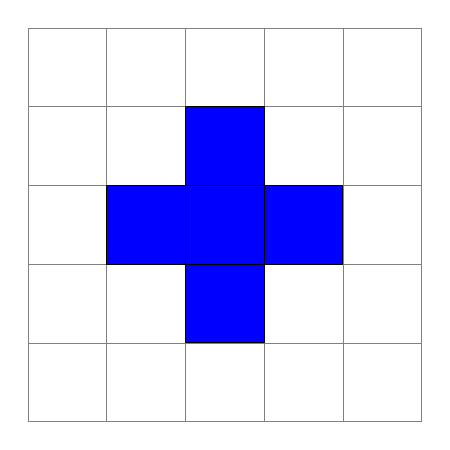
\begin{tikzpicture}
\draw[step=1cm,gray,very thin] (0,0) grid (5,5);
\foreach \x in {-1, 0, 1}
    \foreach \y in {-1, 0, 1}
        \ifthenelse{\x=0 \OR \y=0}{
        \draw[fill=blue]  (2 + \x,2 + \y,0) -- (2+1 + \x,2 + \y,0) -- (2+1 + \x,2+1 + \y,0) -- (2 + \x,2+1 + \y,0) -- cycle; 
        }{};
\end{tikzpicture} 
\end{center}

\pagebreak
\section{Connected island problem 9 directions}
\begin{lstlisting}[
mathescape,
columns=fullflexible,
basicstyle=\fontfamily{lmvtt}\selectfont]

        // eight or nice directions, h = 0 or w = 0 can be ignored in the loop
        count8 arr2d h w height width
            sum = 0
            if arr2d[h][w] is 1
                arr2d[h][w] = 1
                for(int hh=0; hh<=1; hh++)
                    for(int ww=0; ww<=1; ww++)
                        if h + hh >= 0 && h + hh < height ||
                           w + ww >= 0 && w + ww < width
                           sum +=count8 arr2d h+hh w+ww height width
            return sum 
\end{lstlisting} 

\begin{center}
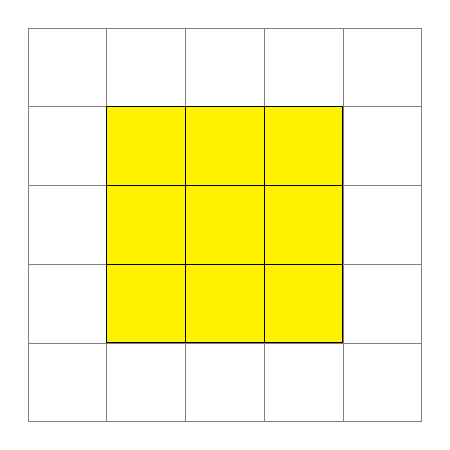
\begin{tikzpicture}
\draw[step=1cm,gray,very thin] (0,0) grid (5,5);
\foreach \x in {-1, 0, 1}
    \foreach \y in {-1, 0, 1}
        \draw[fill=yellow]  (2 + \x,2 + \y,0) -- (2+1 + \x,2 + \y,0) -- (2+1 + \x,2+1 + \y,0) -- (2 + \x,2+1 + \y,0) -- cycle; 
\end{tikzpicture} 
\end{center}

\section{Sudoku Solver}
\subsection{BackTracking}
BackTracking is general algorithm for finding all/some solutions to contraint satisfaction problems,
that incrementally builds candidates to the solution, and abandons each partial c[backtracks] as soon
as it determines that $c$ cannot be possibly completed to a valid solution. \\

For Sudoku problem, the constraint/restriction is row/column and $3\times3$ square have no duplicated number from 1 to 9.
If the number is not valid candidates, reset the cell to previous value and return back to parent. 
\begin{itemize}
\item[] Check Row and Column have no duplicated number 
\item[] Check each $3\times3$ square has no duplicated number 
\item[] Try an empty cell with 1 to 9 
\item[] If the number is valid in the cell, then recur to next empty cell
\item[] Otherwise, set the cell to original value and return back to parent
\end{itemize}

\begin{lstlisting}[
mathescape,
columns=fullflexible,
basicstyle=\fontfamily{lmvtt}\selectfont,
]

    solver arr index
        c = index / 9, r = index % 9
        if index == 9*9
            print arr
        else
            for i 1 to 9
                if arr[c][r] == 0     
                    if checkRowCol arr c r i && checkSquare arr c r i
                        arr[c][r] = i
                        solver arr index + 1
                        arr[c][r] = 0
                else
                    solver arr index + 1

    checkRowCol arr int c int r int n
        for i 0 to 9 
            if arr[c][i] == n || arr[i][r] == n
                return false
        return true

    checkSquare arr c r n
        ic = c/3 ir = r/3
        for c 0 to 3 
            for r to 3 
                arr[c + 3*ic][r + 3*ir] == n
                    return false
        return true
        
\end{lstlisting} 

\section{Eight Queen}
Eight Queen problem is similar Sudoku problem, and can be solved with Backtracking algorithm
The constraint satisfaction is simpler than Sudoku.
\subsection{Runtime is $\mathcal{O}(8^n)$}

\begin{itemize}
\item[] Check whether a queen is in the same column as all other queens 
\item[] Check whether a queen is in the same main diagonal or minor diagonal with all other queens
\end{itemize}

\begin{itemize}
\item[] No two queens are on the same row or column
\item[] Recur down each row 
\item[] If a cell is valid, then go to next row 
\item[] Otherwise, reset the cell and return back to parent/previous call
\end{itemize}

\begin{lstlisting}[
mathescape,
columns=fullflexible,
basicstyle=\fontfamily{lmvtt}\selectfont,
]
    eightQueen
\end{lstlisting} 
\section{Permutation}

\begin{enumerate}
\item Networking
\begin{itemize}
 \item Three ways hands shake 
 \item slide window inside the package
 \item DNS, resolve domain name, IP
 \item TCP, UDP, HTTPS
\end{itemize}

\item Design
\begin{itemize}
 \item load balance
 \item DB replication
 \item Sub-Pub 
 \item command pattern
 \item visit pattern
 \item Singleton, 
 \item Double-checked locking 
 \item message queue
 \item consume and producer
\end{itemize}

\item Quick Sort 
    \begin{itemize}
    \item The average runtime is $\mathcal{O}(n\log{}n)$
    \item The worst case is $\mathcal{O}(n^2)$
        \begin{itemize}
        \item Given an array $[1, 2, 3, 4]$, choose the right most element as \\ 
              pivot which is [4] $=>$ [1, 2, 3][4] $=>$ [1, 2][3] $=>$ [1][2]
        \item How to choose the pivot is critical.
        \end{itemize} 

    \item Memory space is $\mathcal{O}(1)$ 
    \item Untable sort and Stable sort

        \begin{itemize}
        \item If the keys keep the same relative orders after keys are sorted \\ 
              then the sort algorithm is stable. Otherwise it is unstable. \\\\
              Sort the second coordinates \\ 
               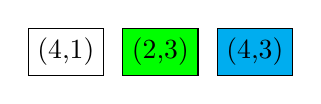
\begin{tikzpicture}
                \coordinate (s) at (0,0);
                  \node[minimum size=6mm, draw, rectangle] at (s) {(4,1)};
                \coordinate (s) at (1.2,0);
                  \node[minimum size=6mm, fill=green, draw, rectangle] at (s) {(2,3)};
                \coordinate (s) at (2.4,0);
                  \node[minimum size=6mm, fill=cyan, draw, rectangle] at (s) {(4,3)};
              \end{tikzpicture} \\

              Sort the first coordinates [stable sort]\\
               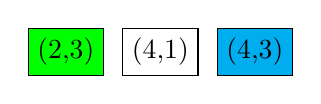
\begin{tikzpicture}
                \coordinate (s) at (0,0);
                  \node[minimum size=6mm, fill=green, draw, rectangle] at (s) {(2,3)};
                \coordinate (s) at (1.2,0);
                  \node[minimum size=6mm, draw, rectangle] at (s) {(4,1)};
                \coordinate (s) at (2.4,0);
                  \node[minimum size=6mm, fill=cyan, draw, rectangle] at (s) {(4,3)};
              \end{tikzpicture} \\

    \item Find the Kth smaller element in a given unsorted array in $\mathcal{O}(n)$

    \item Merge Sort, 
        \begin{itemize}
        \item The average and worst runtime is $\mathcal{O}(n\log{}n)$ 
        \item Stable sort
        \end{itemize} 
    \item Max distance for $j - i$ given $arr[j] > arr[i$] 
    \item Single linked list
    \begin{itemize}
        \item reverse, iteration, recursion
        \item remove, 
        \item insert to sorted list 
        \item clone list
        \item check circular linkedlist 
    \end{itemize} 
    \item Double linkedlist
        \begin{itemize}
            \item remove node
            \item insert node
            \item append node
        \end{itemize} 
    \item Eight queen problem
    \item Sudoku Solver problem
    \item Connected island 
    \item Implement heap with array
    \begin{itemize}
     \item Heap with array \\ 
        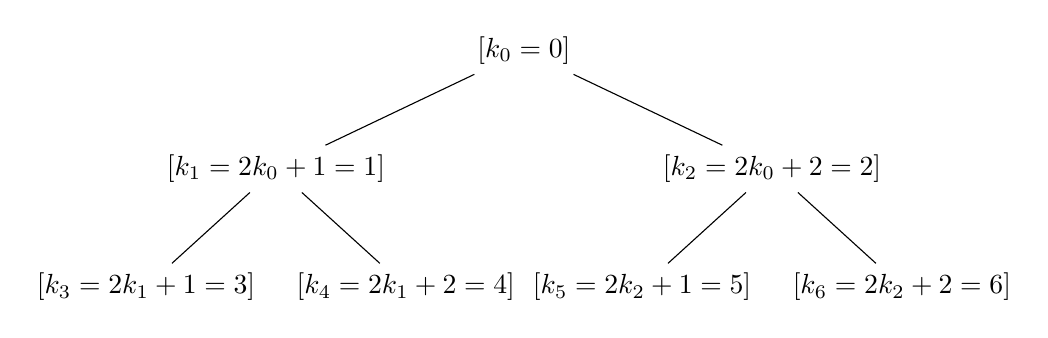
\begin{tikzpicture}[level distance=1.5cm,
        level 1/.style={sibling distance=6.3cm},
        level 2/.style={sibling distance=3.3cm}]
        \node {[$k_0 = 0$]}
        child {node {[$k_1 = 2k_0+1=1$]}
        child {node {[$k_3 = 2k_1+1=3$]}}
        child {node {[$k_4 = 2k_1+2=4$]}}
        }
        child {node {[$k_2 = 2k_0+2=2$]}
        child {node {[$k_5 = 2k_2+1=5$]}}
        child {node {[$k_6 = 2k_2+2=6$]}}
        };
        \end{tikzpicture} 
    \end{itemize}

    \pagebreak
    \item Serialize Binary Tree 
        \begin{itemize}
        \item Use technic similar to the implementation of Heap with array  
            level nodes \\ 
            \[ 2^0 + 2^1 + \dots + 2^k \]
            \[ 2^{k-1}  = 1, 2\]

            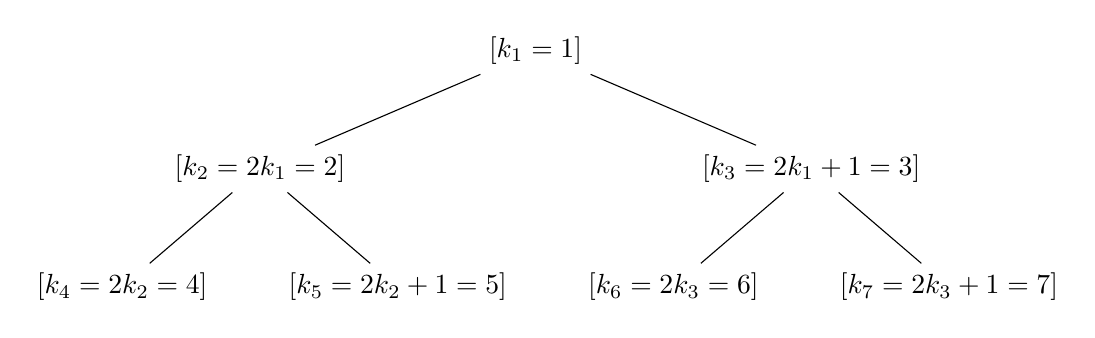
\begin{tikzpicture}[level distance=1.5cm,
            level 1/.style={sibling distance=7cm},
            level 2/.style={sibling distance=3.5cm}]
            \node {[$k_1 = 1$]}
            child {node {[$k_2 = 2k_1=2$]}
            child {node {[$k_4 = 2k_2=4$]}}
            child {node {[$k_5 = 2k_2+1=5$]}}
            }
            child {node {[$k_3 = 2k_1+1=3$]}
            child {node {[$k_6 = 2k_3=6$]}}
            child {node {[$k_7 = 2k_3+1=7$]}}
            };
            \end{tikzpicture} 

            \begin{center}
            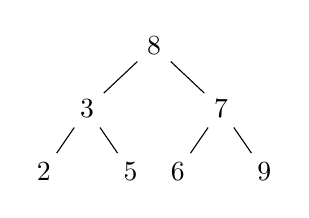
\begin{tikzpicture}[level distance=0.8cm,
            level 1/.style={sibling distance=1.7cm},
            level 2/.style={sibling distance=1.1cm}]
            \node {8}
            child {node {3}
            child {node {2}}
            child {node {5}}
            }
            child {node {7}
            child {node {6}}
            child {node {9}}
            };
            \end{tikzpicture} 
            \end{center}
    \begin{verbatim}
    // [0 : 8] [1 : 3] [2 : 7] [3 : 2] [4 : 5] [5 : 6] [6 : 9]
    level_serial(Node root, int index, String file){
        if(root != null){
            try{
            BufferedWriter bf = new BufferedReader(new FileWriter(file)); 
                bf.write(index + ":" + root.data + "\n");
                level_serial(root.left, 2*index+1, file);
                level_serial(root.right, 2*index+2, file);
            }catch(IOException e){
                e.printStackTrack();
            }
            
        }
    }

    Map<Integer, Integer> createMap(String file){
        BufferedReader bufr = new BufferedReader(FileReader(file));         
        Map<Integer, Integer> map = new HashMap<>();
        String line;
        try((line = buf.readLine()) != null){
            String[] arr = line.split(":");
            map.put(arr[0], arr[1]);
        }catch(IOException e){
            e.printStackTrack();
        }
        return map;
    }
    // index = 0;
    Node buildTree(Map<Integer, Integer> map, int index){
        Node r = null;
        Integer n = map.get(index); 
        if(n != null){
            r = new Node(n);
            r.left = buildTree(map, index + 1);
            r.right = buildTree(map, index + 2);
        }
        return rk;
    }

    \end{verbatim} 
    \end{itemize} 
    \item Rotate square array

    \item Serialize general tree 
    \item Tree Traveral
        \begin{itemize}
        \item preorder  
            \begin{itemize}
            \item pretty print
            \item use it to serialize Binary Tree, postorder can be deserialized BT.
            \end{itemize} 
        \item inorder 

            \begin{itemize}
            \item Check if a Binary Tree is Binary Search Tree   
            \end{itemize} 

        \item postorder
        \begin{itemize}
         \item deserialize  
        \end{itemize}

        
        \item levelorder 
            \begin{itemize}
             \item use two queues 
             \item one queue for odd level
             \item other queue for even level
            \end{itemize}
        \item print level without queues
        \begin{itemize}
         \item compute the height of of the Binary Tree 
         \item $Node(k) = 2^{k-1} \quad k = 1 , \dots , n$
         \begin{verbatim}
            level(Node root, Map<Integer, Integer> map, int index){
                if(root != null){
                    mpa.put(index, root.data);
                    print(root.data);
                    level(root.left, 2*index)
                    level(root.right, 2*index + 1)
                }
            } 

            void printLevel(Map<Integer, Integer> map){
                int count = 0;
                int size = 0;
                while(size < map.size()){
                    int m = (int)Math.pow(2, k);
                    for(int i=1; i<=m; i++){
                        Integer n = map.get(count + i);
                        if(n != null){
                            print(n.data);
                            size++;
                        }
                    }
                    count += m;
                }
            }

            Node buildTree(Map<Integer, Integer> map, int index){
                Node r = null;
                Integer n = map.get(index);
                if(n != null){
                    r = new Node(n);
                    r.left = buildTree(map, 2*index);
                    r.right = buildTree(map, 2*index + 1);
                }
                return r;
            }
         \end{verbatim} 
        \end{itemize}

        \item iteration preorder, inorder, postorder, levelorder
        \item iteration preorder
        \begin{itemize}
        \item initialize $r = root$, stack
        \item iterate left children with $r$ and push the $r$ to stack, at the same time printing out the data 
        \item if $r$ is null, then pop a node from the stack and set the curr reference to the right child of the node 
        \item it will terminate if $r$ is null and stack is empty
        \end{itemize}
         \begin{verbatim}
         preorder(Node r){
             if(r != null){
                 r.data
                 preorder(r.left)  // implicitly r = r.left
                 preorder(r.right) // implicitly pop() => r = r.right
             }
         }

        preorderIte(Node r) {
            Stack<Integer> stack = new Stack<>();
            while(r != null || !stack.isEmpty()) {
                if(r != null) {
                    print(r.data)
                    stack.push(r)
                    r = r.left
                } else {
                    Node n = stack.pop()
                    r = n.right
                }
            }
        }
        \end{verbatim} 

        \pagebreak
        \item iteration inorder
        \begin{itemize}
         \item xxx 
         
         \begin{center}
         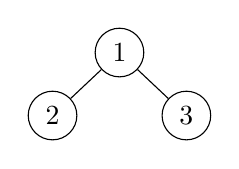
\begin{tikzpicture}[level distance=0.8cm,
         level 1/.style={sibling distance=1.7cm},
         level 2/.style={sibling distance=1.1cm}]
         \node [minimum size=6mm, draw, circle]{1}
         child {node[minimum size=6mm, draw, circle] {2}}
         child {node[minimum size=6mm, draw, circle] {3}};
         \end{tikzpicture} 

         \begin{tabular}{|c|c|c|c|c|c|c|c|c|} \hline
         0      & 1          & 2                 & 3     & 4               & 5          & 6              & 7               \\ \hline
         r=root & $r \arr l$ & $r \arr l \arr l$ & null  & $2 \arr l$=null & $1 \arr r$ & $3\arr l$=null & $3 \arr r$=null \\ \hline
         stack  & push 1     & push 2            & pop 2 & pop 1           & push 3     & pop 3          & x               \\ \hline
         print  & x          & x                 & 2     & 1               & x          & 3              & x               \\ \hline
         \end{tabular} 
         \end{center} 
        \begin{verbatim}
        inorder(Node r){
            if(r != null){
                inorder(r.left)  // => r = r.left, push to stack
                print(r.data)    // => pop(), print(r.data)
                inorder(r.right) // => r = r.right
            }
        }

        inorderIte(Node r){
            Stack<Node> stack = new Stack<>();
            while(r != null || !stack.isEmpty()){
                if(r != null){
                    stack.push(r)
                    r = r.left
                }else{
                    Node n = stack.pop();
                    print(n.data)
                    r = n.right
                }
            }
        }

         \end{verbatim} 
        \end{itemize}
        \item iteration postorder
        \begin{verbatim}
        postorderIte(Node r){
            Stack<Node> s1, s2 = new Stack<>();
            if(r != null){
                s1.push(r);
                while(!s1.empty()){
                    Node top = s1.pop();
                    if(top.left != null)
                        s1.push(top.left);
                    if(top.right != null)
                        s1.push(top.right);

                    s2.push(top);
                }

                while(!s2.empty())
                    s2.pop()
            }
        }
        \end{verbatim} 

        \begin{figure}
        \centering
        \includegraphics[scale=0.2]{/Library/WebServer/Documents/zsurface/image/postorder2.png}
        \caption{Iteration postorder traveral with two stacks}
        \end{figure} 

        \end{itemize}
\end{itemize} 

\item[] level order sequence with two stacks
\item Use two stacks $\arr $ print Binary Tree in sequency order 
     \begin{verbatim}
    public static void printSequence(Node r){
       Stack<Node> s1, s2  = new Stack<>()  
       if(r != null){ 
           s1.push(r)
           while(!s1.empty() || !s2.empty()){
               while(!s1.empty()){
                   Node n = s1.pop()
                   Print.p(n.data)
                   if(n.left != null)
                       s2.push(n.left)
                   if(n.right != null)
                       s2.push(n.right)
               }
               while(!s2.empty()){
                   Node n = s2.pop()
                   Print.p(n.data)
                   if(n.right != null)
                       s1.push(n.right)
                   if(n.left != null)
                       s1.push(n.left)
               }
           }
       }
    }
\end{verbatim} 
\pagebreak
\begin{figure}
\centering
\includegraphics[scale=0.4]{/Users/cat/myfile/github/graphviz/two_stack.pdf}
\caption{two{\_}stack.gv}
\end{figure} 

\item Print rectangle array in spiral shape.
\item Multiply long integers using array 
\item Find the maximum elements from sorted array are shifted
\item Find the minimum elements from sorted array are shifted
\item Merge sorted arrays
\item Merge k sorted arrays
\item Maximum and minimum heap
\item Print n prime and prime number 
\item Use array to represent heap
    \begin{itemize}
     \item The technic can be used to serialize and deserialize Binary Tree
        \end{itemize}

\item heap sort
\item Dynamic Programming
    \begin{itemize}
     \item maximum continuous sum in $\mathcal{O}(n)$ 
     \begin{itemize}
     \item how to support negative number
     \item print the indexes out 
     \end{itemize}
     \item maximum non-continuous sum $\mathcal{O}(n)$ 
     \item multiply all the elements in an array except current element $\mathcal{O}(n)$ 

    \end{itemize}

\item Graphic Problem
\begin{itemize}
 \item Graph
 \item find a path from two nodes (Use Breadth First Search)
 \begin{enumerate}
  \item Check if the n1 and n2 are equal 
  \item if n1 and n2 are equal. we are done!
  \item if n1 and n2 are not equal. 
  \item add n1 to a list
  \item get the first child of n1 and recur with the child.
 \end{enumerate}

 \item find the shortest path from two nodes
 \item find the minimum weight path from two nodes
 \item how to find the loop in a graph
 \item find all the neighbours which are kth distance from a given node
\end{itemize}

\item How to represent a Graph
\begin{itemize}
 \item adjecent matrix 
 \item adjecent list
 \item What is the different between the two data structures
\end{itemize}

\item BackTracking
    \begin{itemize}
     \item Coin Change problem.
     \item Connected island Problem.
     \begin{itemize}
      \item find the minimum number of coins [shortest path from the root]
      \item find the maximum number of coins [longest path from the root]
      \item dynamic programming with HashMap 
     \end{itemize}
     \item Eight Queen Problem
     \item Sudoku Solver
     \item Find the maximum number of connected dots in an 2d array 
     \item Find the path from one word to other word that you can change one letter to a valid word in dictionary only once for each step.
     (Facebook question) 
     \begin{itemize}
      \item Use Depth First Search, DFS
      \item Given two word1 and word2 and a dictinary
      \item start from the first word
      \item change the first position $word[0]$ from $[a-z]$
      \item if the new word is a valid word in the dictionary
      \item move to second position and test $[a-z]$ recursively
      \item if try all possible words from $[a-z]$ and non of them are valid word
      \item return back to the previous recursive call and try the next letter
      \item until the second word2 is found.
      \item otherwise, there is no path from word1 to word2
     \end{itemize}
    
    \end{itemize}

\item Binary Tree
\item Check a Binary Tree is Binary Search Tree 
\item recursion technic
\item defintion technic 
\item Check whether two Binary Tree are isomorphic
\item Find the mirror of a Binary Tree
\item Find the longest path in a Binary Tree
\item Print all the paths in a Binary Tree
\item Find the maximum sum of path in a Binary Tree
\item Invert a Binary Tree
\item Binary Tree to linkedlist

\item Binary Tree to circular double linked list [hard]
\item Binary Tree to single linked list with one queue
\item Delete whole tree
\item Delete whole tree
\item Delete whole tree

\item Use two queues 
\item Post order traveral
\item Use memory space $\mathcal{O}(1)$

\item Move one branch to branch 
\end{itemize}

\item Lease Recent Used[LRU] 
\item Implements HashMap  
\begin{itemize}
 \item Context Switch invoke switching reg, stack pointer, program counter  
\end{itemize}


\begin{itemize}
 \item Synchronize LinkedList 
 \begin{itemize}
  \item $\color{red}{add()}$ and $\color{red}{delete()}$  
  \item Use two locks
  \begin{itemize}
   \item if the node is a head, lock it and delete it, easy!
   \item if the node is not head, then lock the previous and current nodes 
   \item if a node is found, delete it
  \end{itemize}
  \item Why it works?
  \begin{itemize}
   \item If the current node is locked, you can delete the next node safely 
   \item If current node is deleted, then previous node must be locked
  \end{itemize}
 \end{itemize}

 \item What is deadlock 
 \item What is starvation 
 \item Mutex is same for Binary Semaphore 
 \item Semaphore is synchronization construct that can be used to provide
       mutual exclusion and conditional synchronization
 \item Context Switch
 \item Singleton, double-checked locking 
 \item Consumer and Producer
 \item Single LinkedList with two locks add() and delete() 
 \item Java concurrent.Atomic library, AtomicInt, AtomicRef 
 \item Compare and Set [CAS]
 \item Thread, Process, Lock, Spinlocks, Mutex, Semaphore, Compare And Set[CAS]
 \item Synchronize delete or add node in LinkedList. when and where to lock
\end{itemize}

\end{enumerate}
\end{document}
